\documentclass[a4paper,10pt]{report}
\usepackage[utf8]{inputenc}


\usepackage{theorem}        %%Lo agregue yo <========================================
\setcounter{secnumdepth}{7}
\newtheorem{theorem}{Theorem}%[section]
\newtheorem{acknowledgement}[theorem]{Acknowledgement}
%\newtheorem{algorithm}[theorem]{Algorithm}
%\newtheorem{axiom}[theorem]{Axiom}
%\newtheorem{case}[theorem]{Case}
%\newtheorem{claim}[theorem]{Claim}
%\newtheorem{conclusion}[theorem]{Conclusion}
%\newtheorem{condition}[theorem]{Condition}
%\newtheorem{conjecture}[theorem]{Conjecture}
%\newtheorem{criterion}[theorem]{Criterion}
%\newtheorem{exercise}[theorem]{Exercise}
%\newtheorem{notation}[theorem]{Notation}
%\newtheorem{problem}[theorem]{Problem}
%\newtheorem{proposition}[theorem]{Proposition}
%\newtheorem{remark}[theorem]{Remark}
%\newtheorem{solution}[theorem]{Solution}
%\newtheorem{summary}[theorem]{Summary}
\newtheorem{definition}[theorem]{Definition}
\newtheorem{example}[theorem]{Example}
\newtheorem{lemma}[theorem]{Lemma}
\newenvironment{proof}[1][Proof]{\textbf{#1.} }{\ \rule{0.5em}{0.5em}}
\newtheorem{corollary}[theorem]{Corollary}

\usepackage{algorithmic}        %%Lo agregue yo <========================================
\newenvironment{algorithm}[1][Algorithm]{\textbf{#1.} }{}


\usepackage{mdframed}
\newmdtheoremenv{theo}{Theorem}

\usepackage{amsmath, amssymb}
\usepackage{graphicx}
\usepackage{caption}
\usepackage{subcaption}

\usepackage[a4paper,left=3.0cm,right=2.5cm,top=2.5cm]{geometry}
%opening
\title{Fusão  e rotação}
\author{Fernando Pujaico Rivera}

\begin{document}

\maketitle

\begin{abstract}
Este trabalho mostra como achar a matriz de transformação $M^{-1}$ de um vetor de aceleração $\mathbf{A}_n$
numa base nova qualquer, a um vetor $\mathbf{A}_c$ descrito em função da base canônica ($\mathbf{A}_c = M^{-1}\mathbf{A}_n$). 


Para achar a matriz $M$ são usados os vetores de gravidade $\mathbf{g}_n$ e $\mathbf{g}_c$
sendo estes referenciados á base nova e a base canônica, respetivamente.
\end{abstract}

\chapter{Introdução}

O objetivo deste trabalho é mostrar como achar a matriz de transformação $M^{-1}$, 
para ser usado com qualquer vetor de aceleração $\mathbf{A}_n$,
numa base nova qualquer, que deba ser transformado a um vetor $\mathbf{A}_c$, na base canônica; 
de modo que $\mathbf{A}_c = M^{-1}\mathbf{A}_n$. 


Para achar a matriz $M$ debem ser usados os vetores de gravidade $\mathbf{g}_n$ e $\mathbf{g}_c$
sendo estes referenciados á base nova e a base canônica, respetivamente. 
O vetor de gravidade $\mathbf{g}_c$ foi obtido ao inicio do analises e
o vetor $\mathbf{g}_n$ é a gravidade quando os sensores se movimentam.
Assim ambos vetores são medidas de um mesmo sensor em diferentes tempos.




\section{cálculo da gravidade}

A gravidade $\mathbf{g}_n$ pode ser obtida diretamente usando os sensores do celular ($\mathbf{g}_{gravity}$).
E também pode ser calculada em direção a partir do giroscópio ($\mathbf{g}_{gyroscope}$)
dado que o modulo da gravidade não muda para cortas distancias. Assim
aplicando fusão de dados podemos afirmar que
\begin{equation}
 \mathbf{g}_n=\alpha ~ \mathbf{g}_{gravity}+ (1-\alpha)~\mathbf{g}_{gyroscope}.
\end{equation}
Onde $\alpha$ é escolhido entre $0 \leq \alpha \leq 1$ a critério do desenhador.

\chapter{Apêndice}


\section{Velocidade de giro sobre um eixo}


\begin{figure}[h!]
\centering
  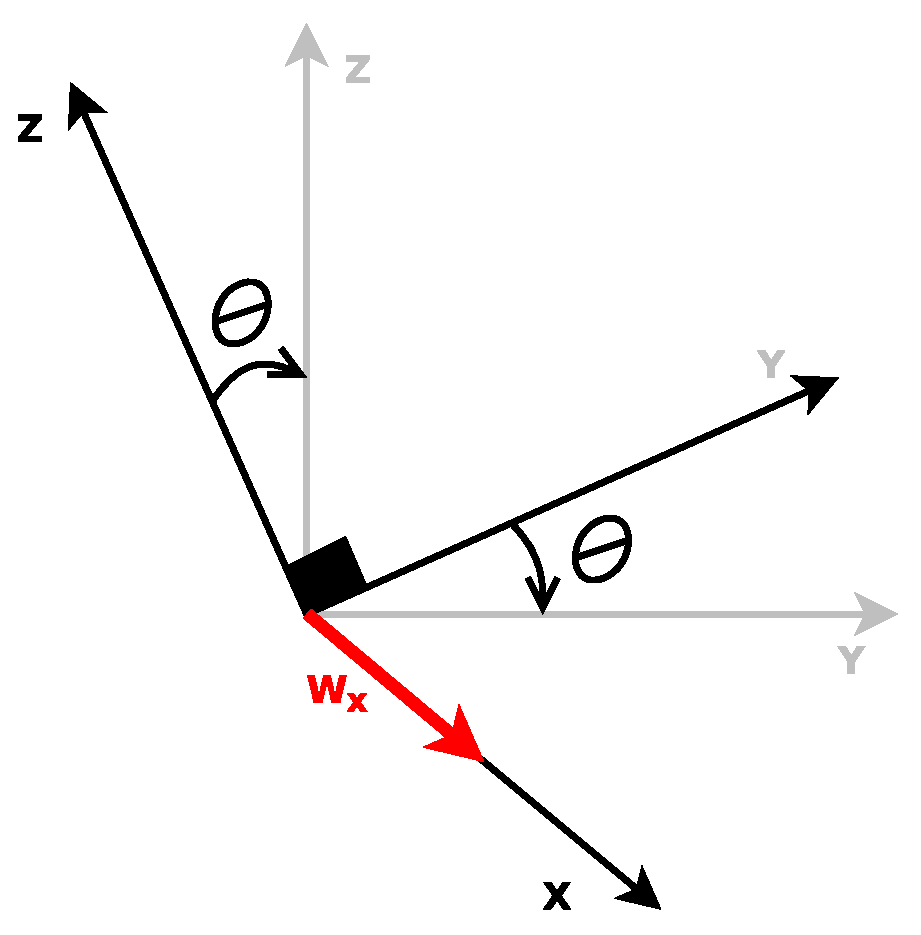
\includegraphics[width=0.3\textwidth]{images/giro.eps} 
\caption{ Velocidade de giro sobre o eixo $\mathbf{X}$}
\label{fig:giro}
\end{figure}
\begin{acknowledgement}\label{acknow:girox}
 A velocidade de giro sobre o eixo $\mathbf{X}$ pode ser representada
 mediante um vetor. No caso da Fig. \ref{fig:giro} pode-se ver que 
 que os eixos coordenados $\{\mathbf{Y},\mathbf{Z}\}$ estão girando de forma horaria
 um angulo $\theta$, tendo como eixo de giro a $\mathbf{X}$.
 Assim define-se a velocidade de giro como o vetor $\mathbf{w}_x \equiv (w_x,0,0)$, onde
 \begin{equation}
  w_x=\frac{d \theta}{d t}.
 \end{equation}
\end{acknowledgement}

\begin{acknowledgement}\label{acknow:giro}
Pode-se generalizar o visto no  Acknowledgement \ref{acknow:girox}, quando temos
um vetor de velocidade de giro $\mathbf{w} \equiv (w_x,w_y,w_z)$.
Este vetor de velocidade de giro pode-se interpretar como se
os eixos coordenados $\{\mathbf{X},\mathbf{Y},\mathbf{Z}\}$ estão girando ao redor
do vetor $\mathbf{e}$ com uma velocidade $w_\mathbf{e}$. Sendo
\begin{equation}
 \mathbf{e}=\frac{\mathbf{w}}{||\mathbf{w}||}
\end{equation}
\begin{equation}
 w_\mathbf{e}=||\mathbf{w}||
\end{equation}

\end{acknowledgement}



\section{Integrando a velocidade de giro}
\begin{acknowledgement}
Conhecendo que os eixos coordenados giram a uma velocidade $w_{\mathbf{e}_i}$
ao redor do vetor $\mathbf{e}_i$ em sentido horário, onde
\begin{equation}
 \mathbf{e}_i=\frac{\mathbf{w}_i}{||\mathbf{w}_i||},
\end{equation}
\begin{equation}
 w_{\mathbf{e}_i}=||\mathbf{w}_i||,
\end{equation}
e $\mathbf{w}_i$ é o vetor de giro no instante $i$.

Se integramos $w_{\mathbf{e}_i}$, obtemos um angulo $\theta_i$ de giro horário dos eixos
ao redor do vetor $\mathbf{e}_i \equiv (e_{w_x},e_{w_y},e_{w_z})$.
Conhecendo o Theo. \ref{theo:girovs} sabemos que um vetor $ \mathbf{v}_i$ na base original
se veria como o vetor  $\mathbf{v}_{i+1}$ na base nova
 \begin{equation}
\mathbf{v}_{i+1} = \mathbf{R}_i \mathbf{v}_i , 
\end{equation}
\begin{equation}
  \mathbf{R}_i = \begin{bmatrix} \cos \theta_i +e_{w_x}^2 \left(1-\cos \theta_i\right) & e_{w_x} e_{w_y} \left(1-\cos \theta_i\right) - e_{w_z} \sin \theta_i & e_{w_x} e_{w_z} \left(1-\cos \theta_i\right) + e_{w_y} \sin \theta_i \\ e_{w_y} e_{w_x} \left(1-\cos \theta_i\right) + e_{w_z} \sin \theta_i & \cos \theta_i + e_{w_y}^2\left(1-\cos \theta_i\right) & e_{w_y} e_{w_z} \left(1-\cos \theta_i\right) - e_{w_x} \sin \theta_i \\ e_{w_z} e_{w_x} \left(1-\cos \theta_i\right) - e_{w_y} \sin \theta_i & e_{w_z} e_{w_y} \left(1-\cos \theta_i\right) + e_{w_x} \sin \theta_i & \cos \theta_i + e_{w_z}^2\left(1-\cos \theta_i\right) \end{bmatrix}. 
\end{equation}

\end{acknowledgement}




\section{Rotação de um vetor ao redor dum eixo}
\begin{acknowledgement}\label{ack:quaterion}


\begin{figure}[h!]
\centering
  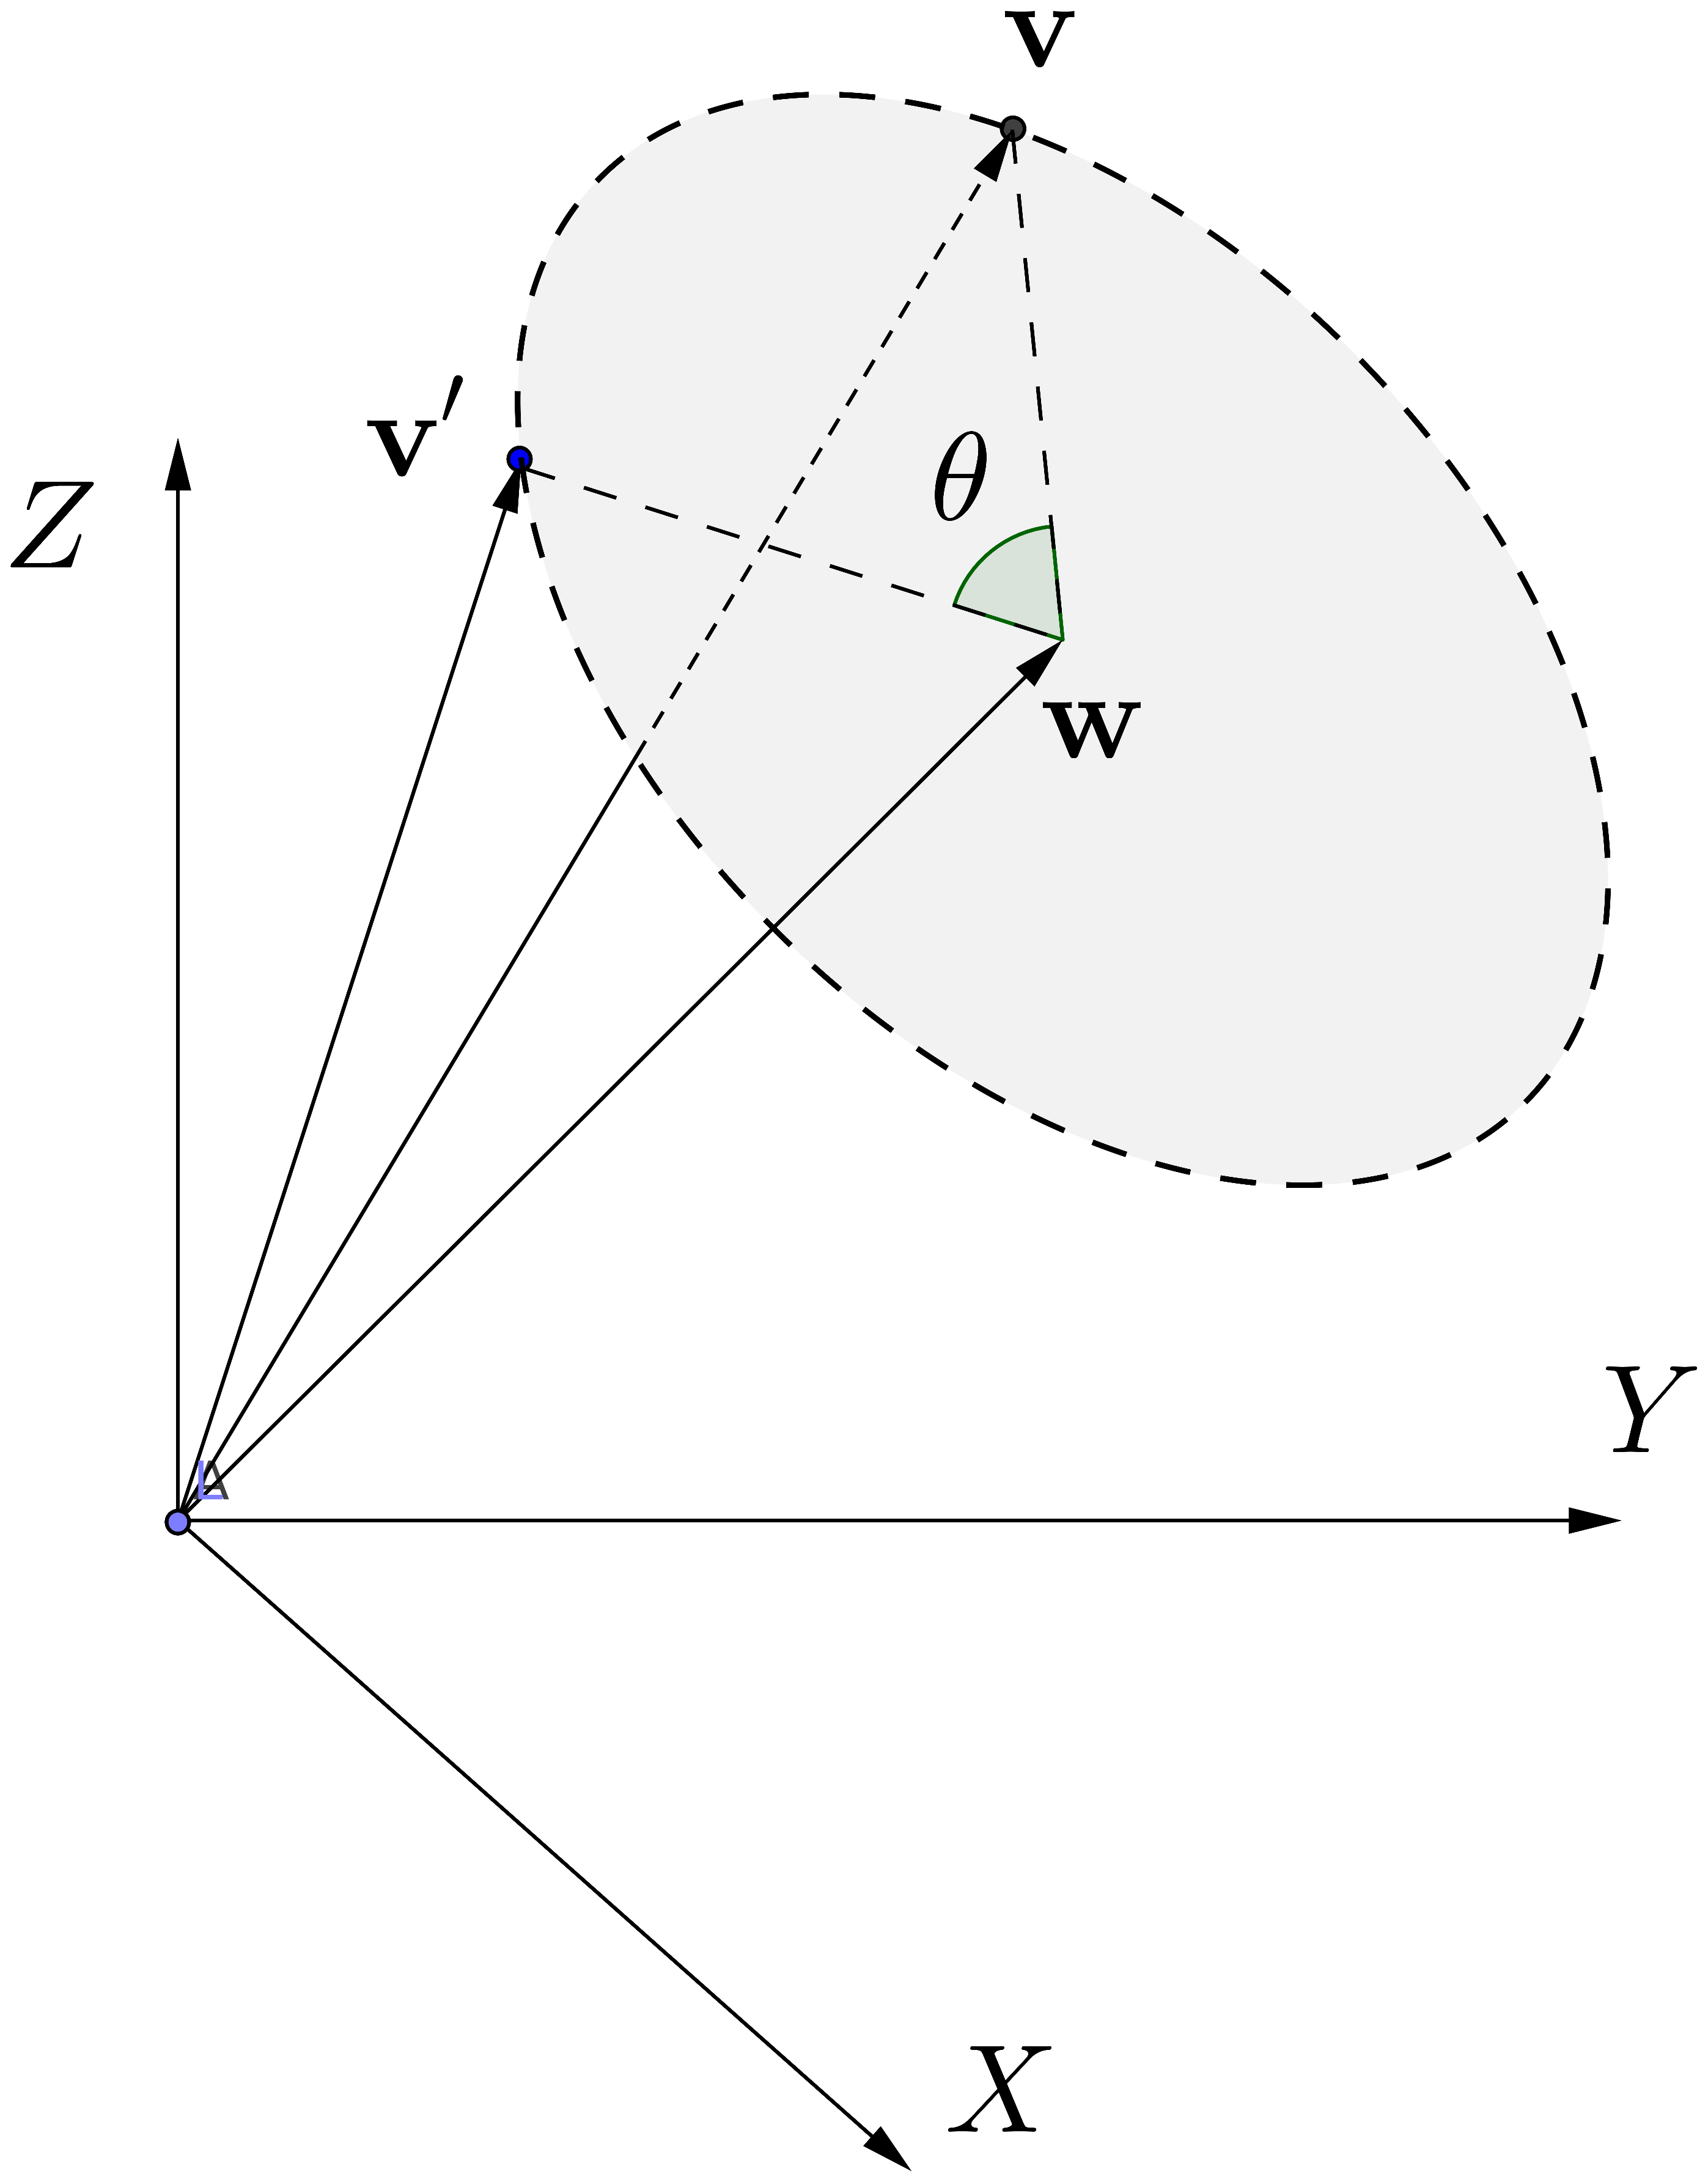
\includegraphics[width=0.3\textwidth]{images/rotaq.eps} 
\caption{ Rotação um angulo $\theta$.}
\label{fig:rotaq}
\end{figure}

 A rotação $\mathbf{v}'=(v_x',v_y',v_z')^T$ de um vetor $\mathbf{v}=(v_x,v_y,v_z)^T$ 
 um angulo $\theta$, em sentido anti-horário, 
 ao redor de um vetor unitário $\mathbf{w}=(w_x,w_y,w_z)^T$, ver Fig. \ref{fig:rotaq}, 
 pode ser compactamente representada através de quaterniões.


\begin{equation}
 V' = Q V Q^{-1},
\end{equation}

onde $Q$ e $W$ são quatérnios de módulo 1
\begin{equation}
Q = \cos \frac {\theta}{2} + \sin \frac {\theta}{2} W,
\end{equation}
\begin{equation}
W=w_x\mathbf{i}+ w_y\mathbf{j}+ w_z\mathbf{k}
\end{equation}
e
\begin{equation}
V=v_x\mathbf{i}+ v_y\mathbf{j}+ v_z\mathbf{k}
\end{equation}
\end{acknowledgement}

\begin{acknowledgement}\label{acknow:giromat}

 A rotação $\mathbf{v}'=(v_x',v_y',v_z')^T$ de um vetor $\mathbf{v}=(v_x,v_y,v_z)^T$ 
 um angulo $\theta$, em sentido anti-horário, 
 ao redor de um vetor unitário $\mathbf{w}=(w_x,w_y,w_z)^T$, ver Fig. \ref{fig:rotaq}, 
 pode ser compactamente representada através de uma matriz.
 
 \begin{equation}
\mathbf{v}' = \mathbf{R} \mathbf{v} , 
\end{equation}
Onde
\begin{equation}
  \mathbf{R} = \begin{bmatrix} \cos \theta +w_x^2 \left(1-\cos \theta\right) & w_x w_y \left(1-\cos \theta\right) - w_z \sin \theta & w_x w_z \left(1-\cos \theta\right) + w_y \sin \theta \\ w_y w_x \left(1-\cos \theta\right) + w_z \sin \theta & \cos \theta + w_y^2\left(1-\cos \theta\right) & w_y w_z \left(1-\cos \theta\right) - w_x \sin \theta \\ w_z w_x \left(1-\cos \theta\right) - w_y \sin \theta & w_z w_y \left(1-\cos \theta\right) + w_x \sin \theta & \cos \theta + w_z^2\left(1-\cos \theta\right) \end{bmatrix}. 
\end{equation}
 
\end{acknowledgement}

\section{Matriz de transformação entre bases}

\begin{figure}[h!]
\centering
  \begin{subfigure}[b]{0.35\textwidth}
  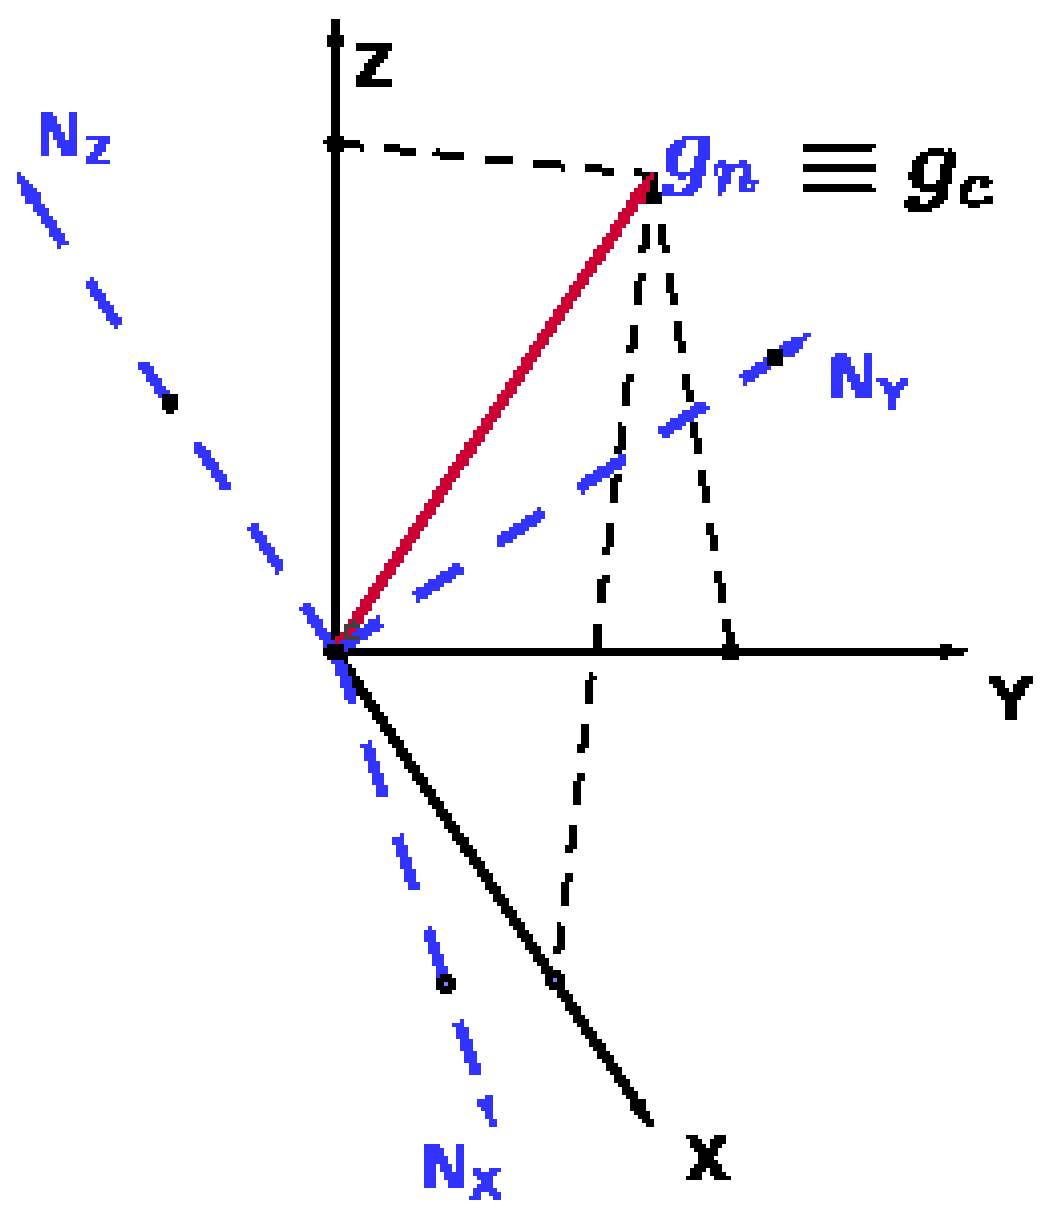
\includegraphics[width=\textwidth]{images/ejes2.eps} 
  \caption{Vetor de gravidade $\mathbf{g}_c$ na base canônica $\{\mathbf{X},\mathbf{Y},\mathbf{Z}\}$.}
  \label{fig:ejes2}
  \end{subfigure}
  \begin{subfigure}[b]{0.35\textwidth}
  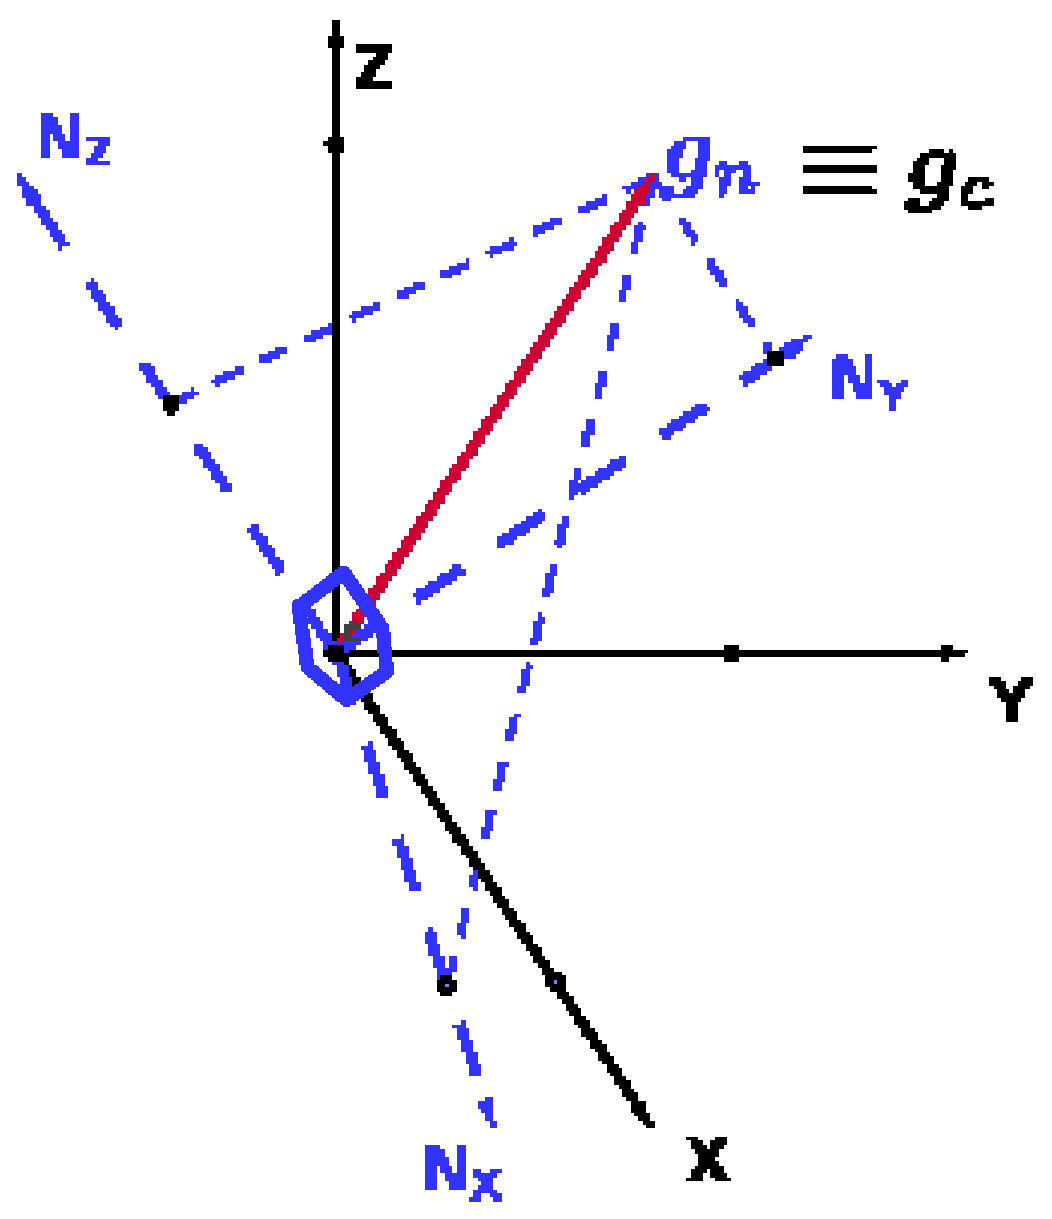
\includegraphics[width=\textwidth]{images/ejes.eps} 
  \caption{Vetor de gravidade $\mathbf{g}_n$ na base nova $\{\mathbf{N}_X,\mathbf{N}_Y,\mathbf{N}_Z\}$.}
  \label{fig:ejes1}
  \end{subfigure}
\caption{ Gravidade referenciado aos eixos canônicos e aos eixos novos.}
\label{fig:ejes}
\end{figure}

\begin{theo}


Dado um vetor $\mathbf{g}_n=(g_{n_x},g_{n_y},g_{n_z})$ em uma base nova qualquer, 
$\{\mathbf{N}_X,\mathbf{N}_Y,\mathbf{N}_Z\}$, e um vetor $\mathbf{g}_c=(g_{c_x},g_{c_y},g_{c_z})$
na base canônica $\{\mathbf{X},\mathbf{Y},\mathbf{Z}\}$, como na Fig. \ref{fig:ejes}, 
A matriz de transformação $M$, onde $M \mathbf{g}_c = \mathbf{g}_n$, é definida
como
\begin{equation}\label{eq:theoM2}
M \equiv \left ( \begin{matrix}
\mathbf{N}_X \\
\mathbf{N}_Y \\
\mathbf{N}_X \times \mathbf{N}_Y \\
\end{matrix}\right).
\end{equation}
onde $\mathbf{N}_X \equiv (n_1 ~ n_2 ~ n_3)$ e $\mathbf{N}_Y \equiv (n_4 ~ n_5 ~ n_6)$.

Para achar estes valores, debe ser definido 
$\mathbf{n}_{i} \equiv (n_1 ~ n_2 ~ n_3 ~ n_4 ~ n_5 ~ n_6)^T$,
de modo que resolvendo a seguinte equação iterativa.
\begin{equation} \label{eq:theoM0}
\mathbf{n}_{0}=(1 0 0 0 1 0)^T,
\end{equation}
\begin{equation} \label{eq:theoM1}
 \mathbf{n}_{i+1}=\mathbf{n}_{i}- \left( \mathbf{J}^T(\mathbf{n}_{i}) \mathbf{J}(\mathbf{n}_{i})\right)^{-1} \mathbf{J}^T(\mathbf{n}_{i}) \mathbf{F}(\mathbf{n}_{i}),
\end{equation}
obtemos o ultimo valor de $\mathbf{n}_{i}$, onde todos estes convergem.
Este valor representará a melhor aproximação para $M$. Os valores das funções matriciais
$\mathbf{F}(\mathbf{n})$ e $\mathbf{J}(\mathbf{n})$ podem ser calculados seguindo a equações (\ref{eq:M2})
e (\ref{eq:M3})

\end{theo}

\begin{proof}
Pode ser achada a matriz de transformação do vetor $\mathbf{g}_c$, 
da base canônica $\{\mathbf{X},\mathbf{Y},\mathbf{Z}\}$ (Fig. \ref{fig:ejes1}),
ao vetor $\mathbf{g}_n$ na base nova $\{\mathbf{N}_X,\mathbf{N}_Y,\mathbf{N}_Z\}$ 
(Fig. \ref{fig:ejes2})
usando a seguinte equação,
\begin{equation}\label{eq:t1}
 M \mathbf{g}_c = \mathbf{g}_n
\end{equation}
Se assumimos que $\{\mathbf{N}_X,\mathbf{N}_Y,\mathbf{N}_Z\}$ são três vetores unitários,
descritos em função da base canônica $\{\mathbf{X},\mathbf{Y},\mathbf{Z}\}$,
então podemos definir a equação anterior como
\begin{equation}\label{eq:t2}
\left ( \begin{matrix}
\mathbf{N}_X \\
\mathbf{N}_Y \\
\mathbf{N}_X \times \mathbf{N}_Y \\
\end{matrix}\right) \mathbf{g}_c = \mathbf{g}_n,
\end{equation}
sendo que $\times$ é o produto crus vetorial.

Assim, também podemos dizer que
\begin{equation}\label{eq:t3}
\mathbf{g}_c = \left ( \begin{matrix}
\mathbf{N}_X \\
\mathbf{N}_Y \\
\mathbf{N}_X \times \mathbf{N}_Y \\
\end{matrix}\right)^{-1}  \mathbf{g}_n = M^{-1}  \mathbf{g}_n
\end{equation}
e consequentemente podemos afirmar que um vetor qualquer $\mathbf{A}_n$,
na base nova, pode ser transformado em $\mathbf{A}_c$, na base canônica
usando
\begin{equation}\label{eq:t4}
\mathbf{A}_c = M^{-1}  \mathbf{A}_n
\end{equation}




Sabemos pela equação (\ref{eq:t1}) e as propriedades dos vetores unitários 
$\{\mathbf{N}_X,\mathbf{N}_Y,\mathbf{N}_Z\}$ que:
\begin{equation}\label{eq:M1}
\mathbf{F}=\left ( \begin{matrix}
\mathbf{N}_X . \mathbf{g}_c - {g}_{n_x}\\
\mathbf{N}_Y . \mathbf{g}_c - {g}_{n_y}\\
(\mathbf{N}_X \times \mathbf{N}_Y) . \mathbf{g}_c - {g}_{n_z}\\
\mathbf{N}_X . \mathbf{N}_Y \\
\mathbf{N}_X . \mathbf{N}_X -1\\
\mathbf{N}_Y . \mathbf{N}_Y -1
\end{matrix}\right)=\mathbf{0} .
\end{equation}

Se definimos $\mathbf{N}_X \equiv (n_1,n_2,n_3)$, $\mathbf{N}_Y \equiv (n_4,n_5,n_6)$ e
$\mathbf{n} \equiv (n_1,n_2,n_3,n_4,n_5,n_6)$
e usamos a equação (\ref{eq:M1}) então é verdade que
\begin{equation}\label{eq:M2}
\mathbf{F}(\mathbf{n})=\left ( \begin{matrix}
n_1 g_{c_x} + n_2 g_{c_y} + n_3 g_{c_z} - g_{n_x} \\
n_4 g_{c_x} + n_5 g_{c_y} + n_6 g_{c_z} - g_{n_y} \\
(n_2 n_6 -n_3 n_5) g_{c_x} + (n_3 n_4 -n_1 n_6) g_{c_y} + (n_1 n_5 -n_2 n_4) g_{c_z} - g_{n_z} \\
n_1 n_4 + n_2 n_5 + n_3 n_6 \\
n_1^2 + n_2^2 +n_3^2 -1 \\
n_4^2 + n_5^2 +n_6^2 -1
\end{matrix}\right)=\mathbf{0} 
\end{equation}
e o jacobiando de $\mathbf{F}(\mathbf{n})$ é
%\tiny
\begin{equation}\label{eq:M3}
\mathbf{J}(\mathbf{n})=\left ( \begin{matrix}
g_{c_x} & g_{c_y} & g_{c_z} & 0      & 0       & 0  \\
0       & 0       & 0       & g_{c_x} & g_{c_y} & g_{c_z} \\
-g_{c_y} n_6 + g_{c_z} n_5  & g_{c_x} n_6 - g_{c_z} n_4 & -g_{c_x} n_5 + g_{c_y} n_4 & g_{c_y} n_3 - g_{c_z} n_2 & -g_{c_x} n_3 + g_{c_z} n_1 & g_{c_x} n_2 - g_{c_y} n_1 \\
n_4     & n_5     & n_6     & n_1    & n_2     & n_3 \\
2 n_1   & 2 n_2   & 2 n_3   & 0      & 0       & 0   \\
0       & 0       & 0       & 2 n_4  & 2 n_5   & 2 n_6   \\
\end{matrix}\right).
\end{equation}
%\normalsize


Utilizando a regularização de Tikhonov, para o caso não lineal, sobre $\mathbf{F}(\mathbf{n})=\mathbf{0} $,
o valor de $\mathbf{n}$ que minimize $\mathbf{F}(\mathbf{n})$ pode ser achado usando
a seguinte equação iterativa
\begin{equation} \label{eq:Tikhonov}
 \mathbf{n}_{i+1}=\mathbf{n}_{i}- \left( \mathbf{J}^T(\mathbf{n}_{i}) \mathbf{J}(\mathbf{n}_{i})\right)^{-1} \mathbf{J}^T(\mathbf{n}_{i}) \mathbf{F}(\mathbf{n}_{i}),
\end{equation}
Onde o simbolo $T$ significa transposta e $\mathbf{n}_0$ poderia ser, por exemplo,
$( 1,0,0, 0,1,0 )$.
\end{proof}

\section{Rotação de eixos versus rotação de pontos }

\begin{figure}[h!]
\centering
  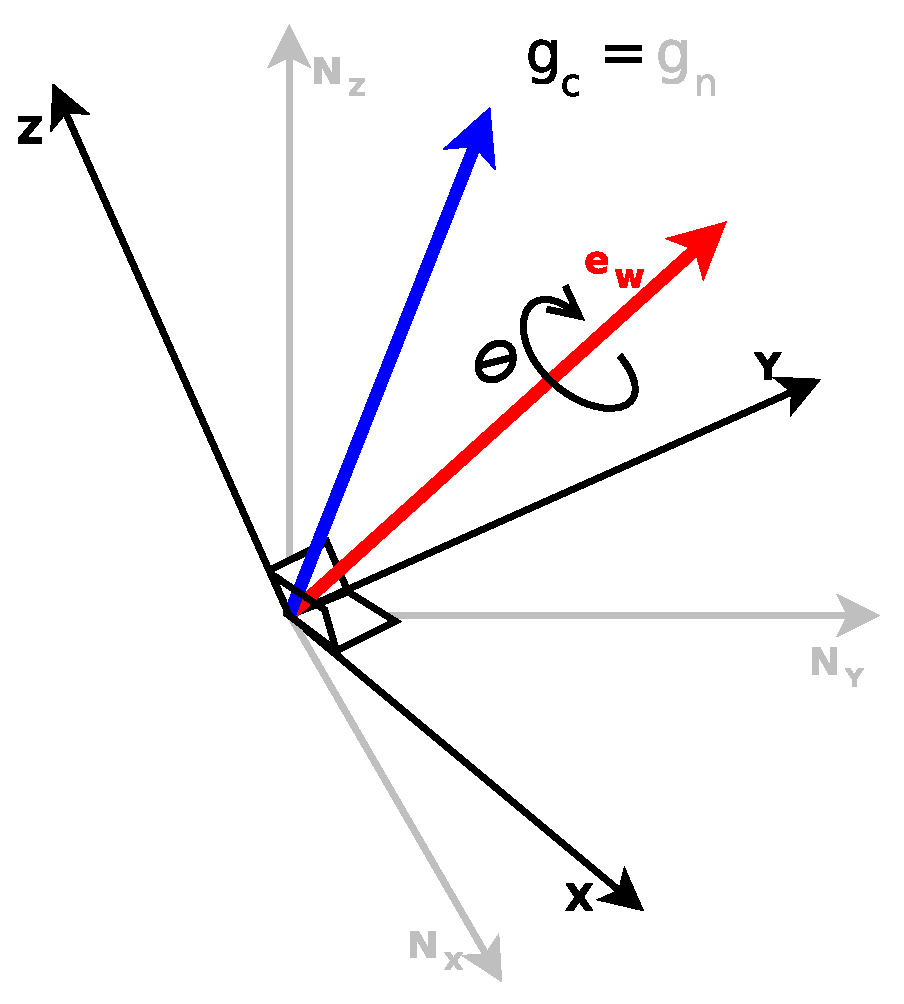
\includegraphics[width=0.3\textwidth]{images/girototal.eps} 
\caption{ Giro dos eixos cordeados um angulo $\theta$.}
\label{fig:girototal}
\end{figure}

\begin{theo}\label{theo:girovs}
 


 Dizer que os eixos giram um angulo $\theta$ em sentido horário ao redor de um 
 vetor $\mathbf{e}_w$, como na Fig. \ref{fig:girototal}, é o mesmo que dizer que um ponto gira um angulo $\theta$ 
 em sentido anti-horário ao redor de um  vetor unitário $\mathbf{e}_w=(e_{w_x},e_{w_y},e_{w_z})$. 
 
 Assim, conhecendo o Acknow. \ref{acknow:giromat}, podemos dizer
 que um vetor $\mathbf{v}$ 
 sofre uma transformação em $\mathbf{v}'$ quando os eixos giram em sentido 
 horário ao redor de um vetor $\mathbf{e}_w$,

 \begin{equation}
\mathbf{v}' = \mathbf{R} \mathbf{v} , 
\end{equation}
Onde
\begin{equation}
  \mathbf{R} = \begin{bmatrix} \cos \theta +e_{w_x}^2 \left(1-\cos \theta\right) & e_{w_x} e_{w_y} \left(1-\cos \theta\right) - e_{w_z} \sin \theta & e_{w_x} e_{w_z} \left(1-\cos \theta\right) + e_{w_y} \sin \theta \\ e_{w_y} e_{w_x} \left(1-\cos \theta\right) + e_{w_z} \sin \theta & \cos \theta + e_{w_y}^2\left(1-\cos \theta\right) & e_{w_y} e_{w_z} \left(1-\cos \theta\right) - e_{w_x} \sin \theta \\ e_{w_z} e_{w_x} \left(1-\cos \theta\right) - e_{w_y} \sin \theta & e_{w_z} e_{w_y} \left(1-\cos \theta\right) + e_{w_x} \sin \theta & \cos \theta + e_{w_z}^2\left(1-\cos \theta\right) \end{bmatrix}. 
\end{equation}
\end{theo}

\begin{proof}
\begin{figure}[h!]
\centering
  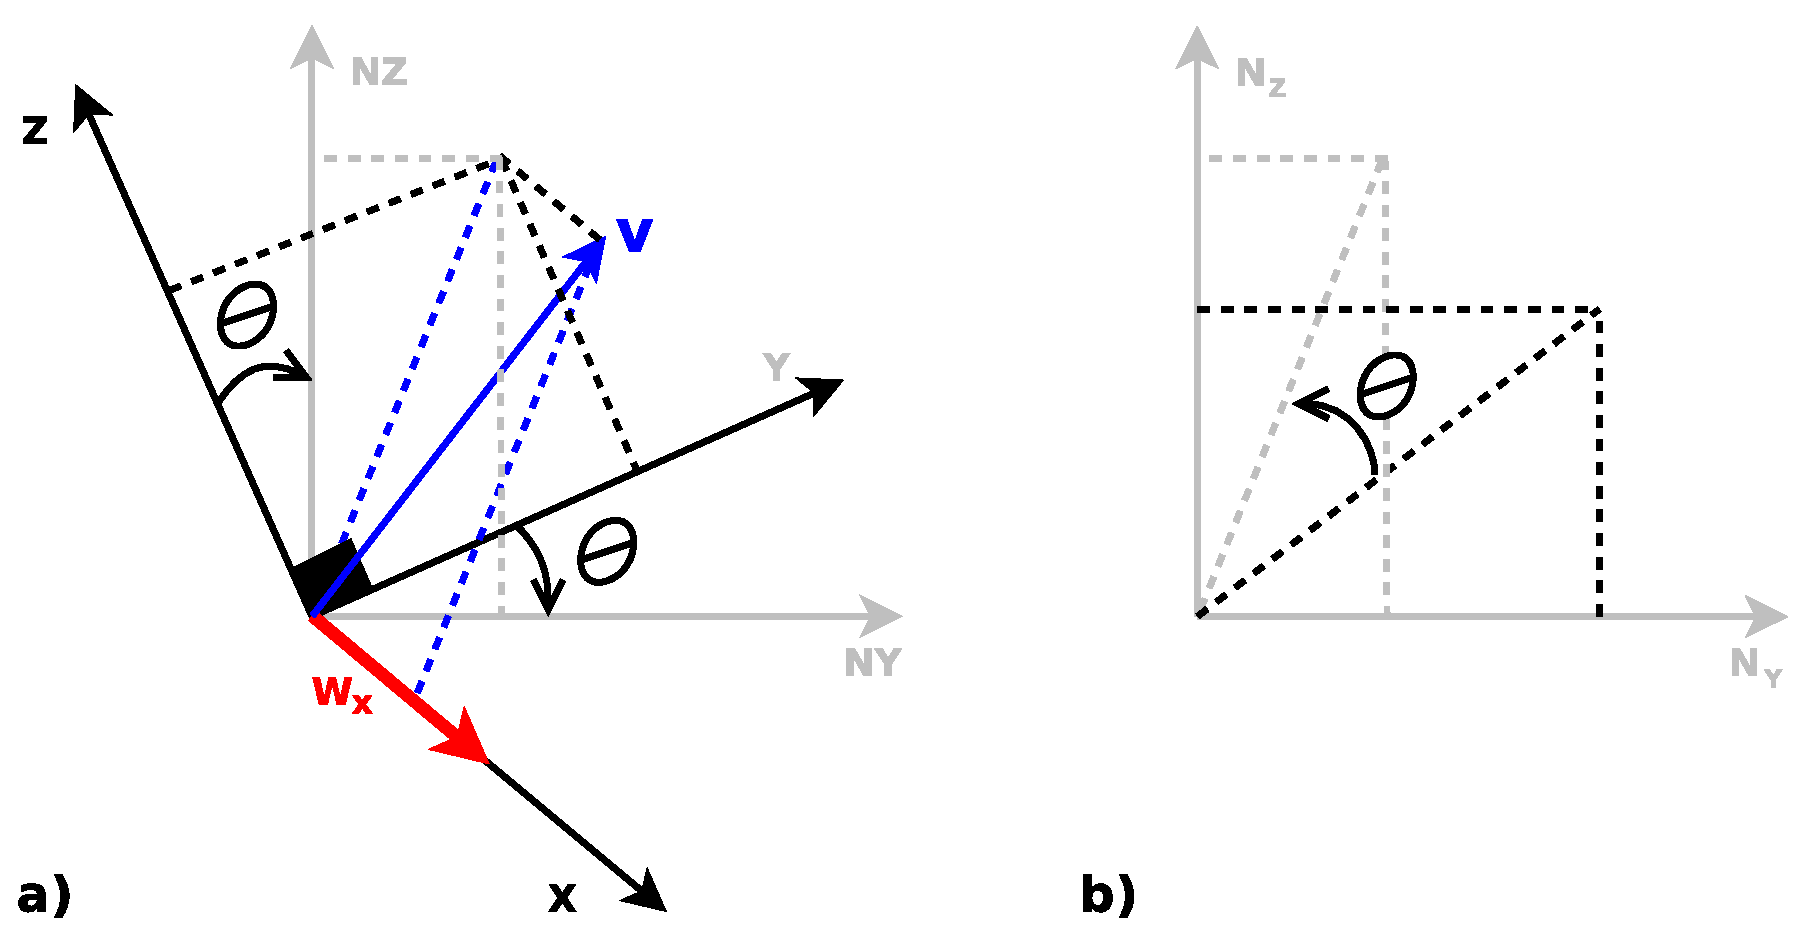
\includegraphics[width=0.8\textwidth]{images/giroparcial.eps} 
\caption{ comparação da perceptiva de giro.}
\label{fig:giroparcial}
\end{figure}
 É fácil de perceber quando analisamos o giro num eixo coordenado
 como na Fig. \ref{fig:giroparcial}a.
 Esta figura mostra como os eixos coordenados
 $\{\mathbf{X},\mathbf{Y},\mathbf{Z}\}$ giram ao redor do eixo 
 $\mathbf{X}$ um angulo $\theta$ no sentido horário.
 Para efeitos de exemplo, se presenta também o vetor $\mathbf{v}$
 e suas distintas projeções no eixo canônico é o eixo girado,
 como pode ser visto na Fig. \ref{fig:giroparcial}b.
 Assim, é fácil de ver que desde o ponto de vista do vetor,
 este gira um angulo $\theta$ em sentido anti-horário.
\end{proof}



\end{document}
